% Native vector artwork. Compile with: pdflatex 03_elastic_hex.tex
% No external graphics, fonts, or data are needed.
% Stylized peristalsis, porous elastic skeleton, and rightward fluid transport.
\documentclass[tikz,border=0pt]{standalone}
\usetikzlibrary{arrows.meta,calc}
\definecolor{navy}{HTML}{193951}
\definecolor{blue}{HTML}{168DA6}
\definecolor{cyan}{HTML}{51D6D0}
\definecolor{coral}{HTML}{E58259}
\definecolor{pale}{HTML}{EAF6F7}
\definecolor{mesh}{HTML}{9EBBC4}
\begin{document}
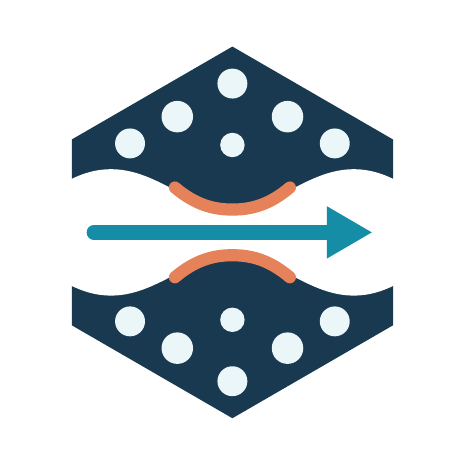
\begin{tikzpicture}[x=1cm,y=1cm,line cap=round,line join=round]
\path[use as bounding box] (-2.6,-2.6) rectangle (2.6,2.6);

% Geometric software-package emblem: elastic porous bands and a flow corridor.
\path[fill=navy]
 (0,2.36) -- (2.04,1.18) -- (2.04,-1.18)
 -- (0,-2.36) -- (-2.04,-1.18) -- (-2.04,1.18) -- cycle;
% Opposing wave surfaces squeeze the white pore-fluid corridor.
\path[fill=white]
 (-2.08,.66) .. controls (-1.18,1.13) and (-.68,.29) .. (0,.29)
 .. controls (.68,.29) and (1.18,1.13) .. (2.08,.66)
 -- (2.08,-.66) .. controls (1.18,-1.13) and (.68,-.29) .. (0,-.29)
 .. controls (-.68,-.29) and (-1.18,-1.13) .. (-2.08,-.66) -- cycle;
% Broad coral segments mark the region of peristaltic compression.
\foreach \s in {-1,1}{
 \begin{scope}[yscale=\s]
  \draw[coral,line width=4.4pt]
    (-.73,.57) .. controls (-.47,.35) and (-.24,.29) .. (0,.29)
    .. controls (.24,.29) and (.47,.35) .. (.73,.57);
  % Pores are negative space in the solid; smaller central pores imply strain.
  \foreach \x/\y/\r in {-1.30/1.13/.19,-.70/1.47/.20,0/1.11/.155,.70/1.47/.20,1.30/1.13/.19,0/1.89/.19}{
   \fill[pale] (\x,\y) circle (\r);
  }
 \end{scope}
}
\draw[blue,line width=5.2pt,-{Triangle[length=5.8mm,width=6.2mm]}]
 (-1.76,0) -- (1.78,0);
\end{tikzpicture}
\end{document}
